
%%
%% INSTRUCOES
%%
%% Imagem Docker para compilar o documento:
%%
%% docker pull texlive/texlive
%%
%% Levantar o container:
%%
%% docker run -it --rm -v "${PWD}:/doc" -w /doc texlive/texlive bash
%%
%% Compilar o documento para PDF:
%%
%% pdflatex relatorio
%% bibtex relatorio
%% pdflatex relatorio
%% pdflatex relatorio
%%

\documentclass[a4paper, 12pt]{article}
%\documentclass[a4paper, 12pt]{report}

%%
%% PACOTES
%%

\usepackage[utf8]{inputenc}
\usepackage[portuguese]{babel}
\usepackage{pdfpages} % incluir ficheiros PDF - para a capa
\usepackage{indentfirst} % identar a primeira linha
\usepackage[nottoc,numbib]{tocbibind} % referencias aparecerem no indice

\usepackage{geometry}
\geometry{margin=2.5cm} % diminuir a margem

%%
%% METADADOS
%%

\title{Relatorio }
\author{Grupo}
\date{\today}

%%
%% INICIO DO DOCUMENTO
%%

\begin{document}

%% CAPA

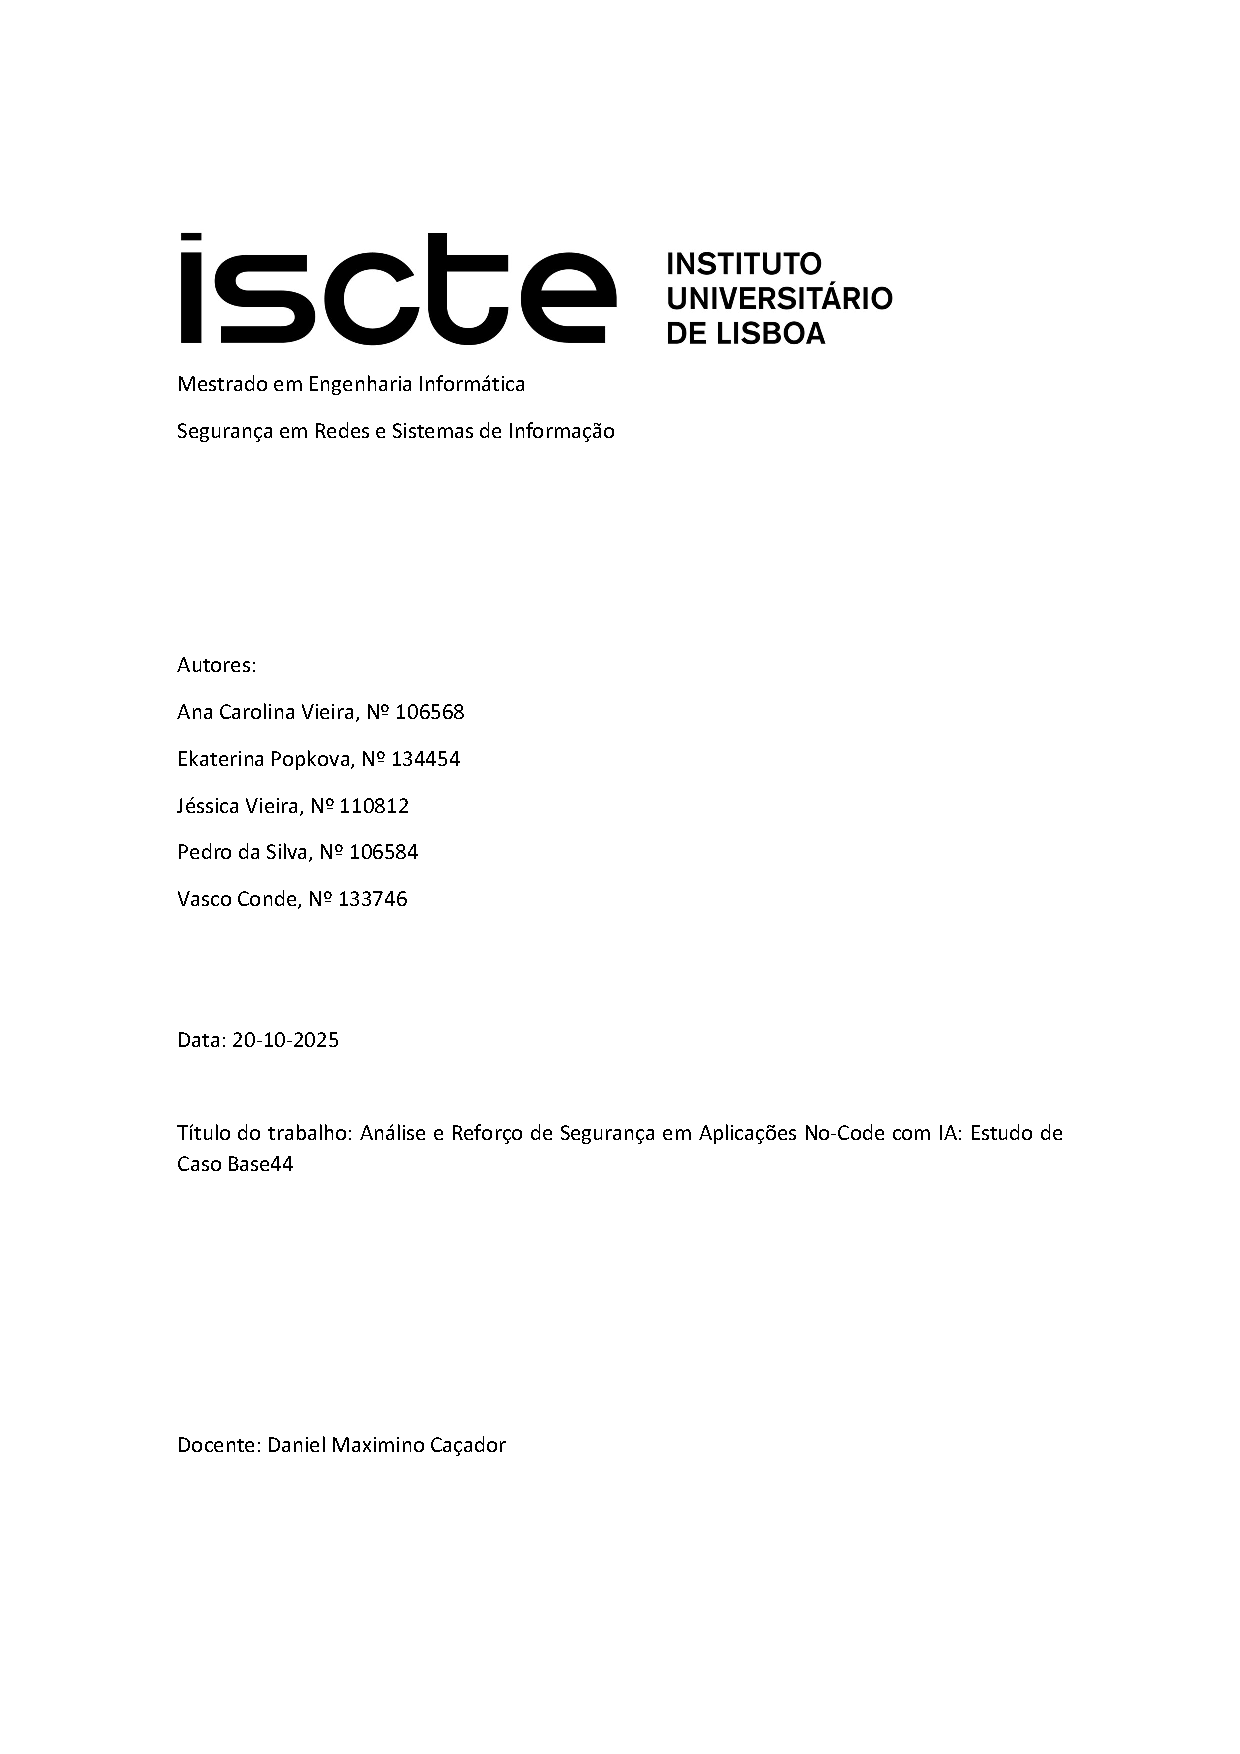
\includepdf{capa/capa.pdf}

%% RESUMO


\begin{abstract}
O presente trabalho tem como objetivo analisar vulnerabilidades de segurança em aplicações desenvolvidas com a plataforma Base44, uma solução no-code baseada em inteligência artificial. A investigação centra-se no código do lado do cliente (frontend), procurando avaliar os riscos que podem existir mesmo sem acesso ao backend da aplicação.

A análise será conduzida segundo uma abordagem de testes de penetração do tipo caixa-cinzenta, adequada a contextos onde o acesso à infraestrutura é limitado. O estudo incidirá sobre falhas detetáveis através do navegador, como o armazenamento inseguro de dados, a manipulação inadequada do DOM e a exposição de recursos sensíveis. 

Com este projeto, pretende-se contribuir para uma maior consciência dos riscos inerentes ao desenvolvimento em plataformas no-code, sublinhando a importância da segurança mesmo em ambientes onde o controlo técnico do programador é reduzido.



\textbf{Keywords}: Segurança Web, Base44, Frontend, Cross-Site Scripting (XSS), LocalStorage, Service Worker.
\end{abstract}

%% INDICES

\tableofcontents

%\listoftables

\listoffigures

% CAPITULOS

\section{Vulnerabilidades Testadas mas Não Detetadas}

Durante a análise de segurança à aplicação alojada na plataforma Base44, foram também considerados outros vetores de ataque comuns em aplicações web modernas, com o objetivo de realizar uma avaliação mais abrangente e alinhada com as boas práticas internacionais de segurança \cite{ref1, ref2}.

Ainda que não tenham sido identificadas ocorrências dessas vulnerabilidades no projeto em análise, a sua inclusão demonstra uma abordagem metodológica informada e coerente com os princípios do OWASP e das normas NIST \cite{ref3, ref4}.

Segue-se o resumo das vulnerabilidades analisadas, precedido por uma breve descrição teórica de cada uma.

\subsection{CORS Mal Configurado (\textit{Cross-Origin Resource Sharing})}

\subsubsection{Enquadramento Teórico}

O \textit{Cross-Origin Resource Sharing} (CORS) é um mecanismo de segurança implementado nos navegadores modernos que controla como recursos (por exemplo, dados de APIs) podem ser solicitados entre diferentes origens (\textit{origins}) \cite{ref5}.

Sem CORS, o \textit{Same-Origin Policy} (SOP) impede que \textit{scripts} executados numa origem (e.g., \url{https://app.example.com}) acedam a recursos noutra (e.g., \url{https://api.example.org}).

Uma configuração incorreta de CORS pode permitir que um domínio malicioso obtenha dados sensíveis através de pedidos legítimos, violando a confidencialidade da aplicação. Exemplos comuns incluem:
\begin{itemize}

\item Cabeçalhos permissivos, como Access-Control-Allow-Origin: *;

\item Reflexão do valor de \textit{Origin} sem validação;

\item Permissão de cabeçalhos ou métodos inseguros.

\end{itemize}

\subsubsection{Análise Realizada}

Foi efetuado um teste manual utilizando o comando cURL com cabeçalhos personalizados de \textit{Origin}, de forma a verificar se o servidor aceitava requisições de domínios externos sem validação adequada.\\

\verb!curl -I -H "Origin: http://malicious.example.com" https://app.base44.io!\\

Durante os testes, não foram detetadas configurações permissivas, nem cabeçalhos vulneráveis. Conclui-se que a aplicação não apresenta fragilidades relacionadas com CORS nesta fase \cite{ref7}.

\subsection{Riscos Associados a \textit{Service Workers e Cache Storage}}

\subsubsection{Enquadramento Teórico}

Os \textit{Service Workers} são \textit{scripts} registados pelo navegador que atuam como \textit{proxies} entre a aplicação e a rede, permitindo funcionalidades como execução \textit{offline}, \textit{background synchronization} e \textit{push notifications} \cite{ref8}.

Embora úteis, podem introduzir riscos de segurança se mal configurados - nomeadamente:

\begin{itemize}

\item \textit{Cache poisoning}, quando conteúdo malicioso é armazenado e servido como legítimo;

\item \textit{Persistent malicious scripts}, que se mantêm mesmo após correções no servidor;

\item Manutenção indevida de dados sensíveis em \textit{Cache Storage}.

\end{itemize}

Uma aplicação que utilize \textit{Service Workers} deve assegurar controlos de integridade, âmbito restrito e atualização segura \cite{ref9}.

\subsubsection{Análise Realizada}

A análise ao código-fonte revelou ausência de qualquer registo ou implementação de \textit{Service Workers} e de uso explícito da \textit{Cache Storage API}, tornando este vetor não aplicável a este projeto em análise.

Consequentemente, os riscos associados a \textit{offline persistence} ou manipulação de \textit{cache} são inexistentes nesta fase.

\subsection{Vulnerabilidades em \textit{Scripts} de Terceiros}

\subsubsection{Enquadramento Teórico}

Bibliotecas e \textit{frameworks} de terceiros são componentes fundamentais no desenvolvimento web, mas também representam um dos principais meios de ataque modernos \cite{ref10}.

Ataques à cadeia de fornecimento (\textit{supply chain attacks}) podem ocorrer quando uma dependência legítima é comprometida, afetando todas as aplicações que a utilizam.

Outros riscos incluem:

\begin{itemize}

\item Inclusão de versões desatualizadas com vulnerabilidades conhecidas (CVE);

\item Hospedagem de \textit{scripts} em CDNs não confiáveis;

\item Modificação de dependências por terceiros não autorizados.

\end{itemize}

A OWASP recomenda o uso de ferramentas de verificação de dependências e auditorias regulares para reduzir esse risco \cite{ref11}.

\subsubsection{Análise Realizada}

Foi conduzida uma inspeção estática e dinâmica aos ficheiros JavaScript utilizados na aplicação, com foco nas dependências externas.

Verificou-se que apenas foram incluídas versões oficiais hospedadas em CDNs reputadas, como jsDelivr e Cloudflare.

Não foram encontradas bibliotecas desatualizadas ou modificadas, reduzindo significativamente o risco de exploração.

\subsection{Exposição de \textit{Tokens} ou API \textit{keys}}

\subsubsection{Enquadramento Teórico}

A exposição de segredos (como \textit{tokens}, API \textit{keys} ou credenciais) é uma das falhas mais comuns em aplicações web e representa uma ameaça direta à integridade e confidencialidade do sistema \cite{ref12}.

Quando segredos estão embutidos no código-fonte — especialmente no \textit{frontend} — tornam-se acessíveis a qualquer utilizador que inspecione o código, permitindo:

\begin{itemize}

\item Autenticação não autorizada em APIs;

\item Acesso a dados confidenciais;

\item Comprometimento de outros serviços integrados.

\end{itemize}

A OWASP recomenda a gestão centralizada de segredos, armazenamento seguro no servidor e rotação periódica de chaves \cite{ref13}.

\subsubsection{Análise Realizada}

Durante a análise estática do código-fonte (HTML, JavaScript e cabeçalhos HTTP), procuraram-se padrões típicos de exposição de segredos, incluindo termos como \textit{apiKey}, \textit{token}, \textit{Authorization}, e chaves codificadas em Base64.

Foram efetuadas pesquisas manuais e automatizadas, incluindo inspeção de ficheiros minificados.

Não foram identificados valores sensíveis embutidos no código, o que demonstra uma boa segregação de segredos e práticas seguras de gestão de credenciais \cite{ref14, ref15}.

\subsection{Conclusão}

Embora nenhuma destas vulnerabilidades tenha sido identificada na aplicação analisada, a sua verificação foi essencial para garantir uma abordagem responsável, abrangente e conforme as normas internacionais de segurança.

Os resultados reforçam que, mesmo em ambientes \textit{no-code} e com integração de IA, é possível seguir metodologias de análise de risco alinhadas com os princípios do OWASP Top 10 (2021) e do NIST Cybersecurity Framework (CSF) \cite{ref2, ref4}.


\section{Questões Conhecidas e Reportadas ao Nível da Plataforma (Base44)}

% BIBLIOGRAFIA

\bibliography{bibliografia/biblio}{}
\bibliographystyle{apalike}

%%
%% FIM DO DOCUMENTO
%%
\end{document}
